\documentclass{article}

\usepackage{tikz}

\begin{document}
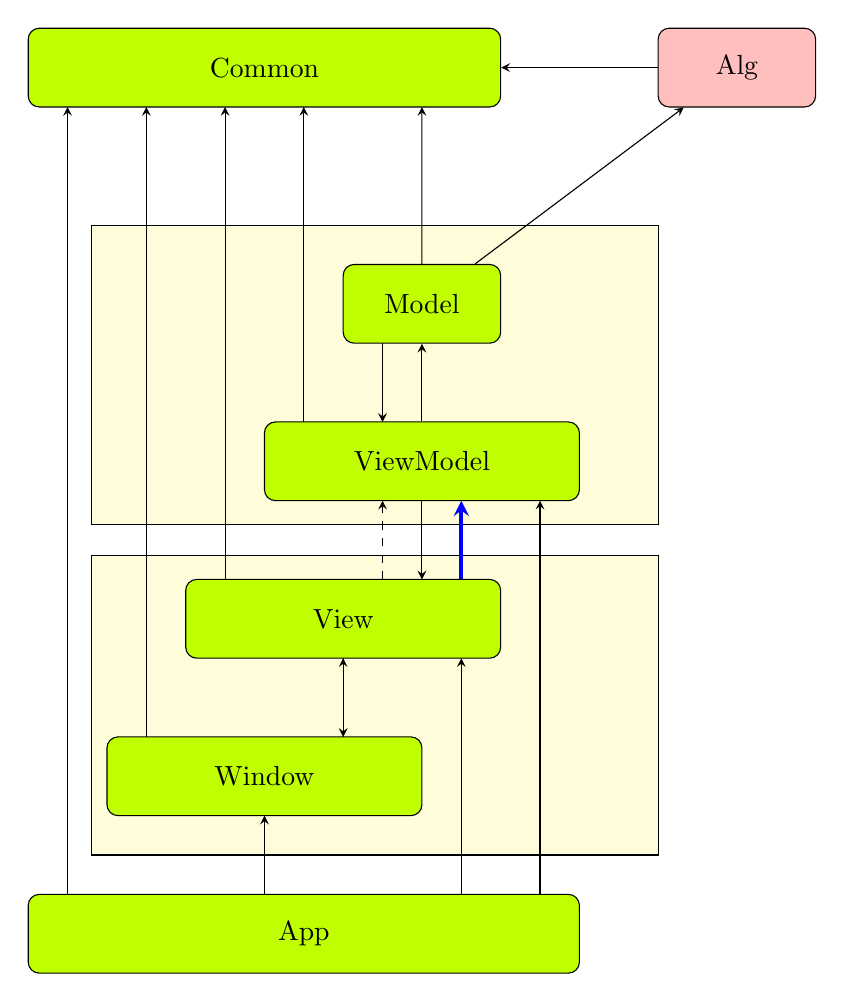
\begin{tikzpicture}
%define
\tikzstyle{state} = [rectangle, rounded corners, minimum width=2cm, minimum height=1cm, text centered, draw=black, fill = pink]
\tikzstyle{state1} = [rectangle, rounded corners, minimum width=2cm, minimum height=1cm, text centered, draw=black, fill = lime]
\tikzstyle{state2} = [rectangle, rounded corners, minimum width=4cm, minimum height=1cm, text centered, draw=black, fill = lime]
\tikzstyle{state3} = [rectangle, rounded corners, minimum width=6cm, minimum height=1cm, text centered, draw=black, fill = lime]
\tikzstyle{state4} = [rectangle, rounded corners, minimum width=7cm, minimum height=1cm, text centered, draw=black, fill = lime]
\tikzstyle{arrow} = [->, >=stealth]
\tikzstyle{arrowb} = [->, >=stealth, blue, line width = 0.05cm]
\tikzstyle{arrowx} = [->, >=stealth, dashed]

%block1
\filldraw[fill = yellow, opacity = 0.15, draw opacity = 1](-2.2,-2)rectangle(5,-5.8);
%block2
\filldraw[fill = yellow, opacity = 0.15, draw opacity = 1](-2.2,-6.2)rectangle(5,-10);

\node[state3, draw, align=left](layer1){Common};
\node[state, right of = layer1, xshift = 5cm, draw, align=left](other){Alg};
\node[state1, below of = layer1, xshift = 2cm, yshift = -2cm, draw, align=left](layer2){Model};
\node[state2, below of = layer1, xshift = 2cm, yshift = -4cm, draw, align=left](layer3){ViewModel};
\node[state2, below of = layer1, xshift = 1cm, yshift = -6cm, draw, align=left](layer4){View};
\node[state2, below of = layer1, yshift = -8cm, draw, align=left](layer5){Window};
\node[state4, below of = layer1, xshift = 0.5cm, yshift = -10cm, draw, align=left](layer6){App};
%line
\draw[arrow](layer2)--(other);
\draw[arrow](other)--(layer1);
\draw[arrow](layer2)--(2,-0.5);
\draw[arrow](0.5,-4.5)--(0.5,-0.5);
\draw[arrow](-0.5,-6.5)--(-0.5,-0.5);
\draw[arrow](-1.5,-8.5)--(-1.5,-0.5);
\draw[arrow](-2.5,-10.5)--(-2.5,-0.5);
\draw[arrow](1.5,-3.5)--(1.5,-4.5);
\draw[arrow](layer3)--(layer2);
\draw[arrowx](1.5,-6.5)--(1.5,-5.5);
\draw[arrow](2,-5.5)--(2,-6.5);
\draw[arrow](1,-7.5)--(1,-8.5);
\draw[arrow](1,-8.5)--(1,-7.5);
\draw[arrowb](2.5,-6.5)--(2.5,-5.5);
\draw[arrow](0,-10.5)--(0,-9.5);
\draw[arrow](2.5,-10.5)--(2.5,-7.5);
\draw[arrow](3.5,-10.5)--(3.5,-5.5);

\end{tikzpicture}
\end{document}